\documentclass[12pt, a4paper]{article}
\usepackage{a4wide}

\usepackage[utf8]{inputenc}
\usepackage[ngerman]{babel}
\usepackage[T1]{fontenc}
\usepackage{palatino} %font

\usepackage{graphicx}
\usepackage{caption}
\usepackage{subcaption} %für subfigures
\usepackage{url}
\usepackage{tocloft}
\usepackage{acronym}
\usepackage{float}
\usepackage{color} 

\usepackage[babel,german=quotes,threshold=3]{csquotes} 

\usepackage{lipsum}
\usepackage{hyperref}  %hyperref still needs to be put at the end!

%Pfad für Grafiken
\graphicspath{{img/}}

%Styleregeln
\widowpenalty10000 % Vermeidet einzelne Zeilen eines Absatzes zu Beginn einer Seite
\clubpenalty10000 % Vermeidet einzelne Zeilen eines Absatzes am Ende einer Seite
\addtocontents{toc}{\protect\sloppy}
\setcounter{tocdepth}{3}

\begin{document}

%deaktiviere Seitenzahlen
\pagenumbering{gobble}

%Titelseite
\begin{titlepage}
\centering
\thispagestyle{empty}
\begin{center}

\includegraphics[width=0.9\textwidth]{uos.pdf}
\end{center}
\LARGE{\textsc{Institut für Informatik\\Arbeitsgruppe Verteilte Systeme}}
\vfill
\LARGE{\emph{Seminar}}\\
\LARGE{\emph{Mobility and Traffic in Computer Networks}}\\
\vspace{8mm}
\huge{\textbf{{\fontfamily{ppl}\selectfont
Mobility-Traffic Correlations}}}\\
\vspace{9mm}
\LARGE{Tim Bohne}\\
\vspace{0.2cm}
%ACHTUNG: !!!Matrikelnummer nur für die Abgabeversion, NICHT mit ins Wiki hochladen!!!
% \normalsize{Matrikelnummer}\\
\vspace{4cm}
\large{Sommersemester 2019}\\
\vspace{0.2cm}
\large{\today}
\vfill
\end{titlepage}
\newpage

%Inhaltsverzeichnis
\tableofcontents
\newpage

\pagestyle{plain}
\pagenumbering{arabic} %Starte Seitennummerierung

\section{Einleitung}

Die stetig wachsende Zahl vernetzter Geräte führt zu enormen Herausforderungen bei der Entwicklung
und Planung der dafür erforderlichen Infrastruktur. Beim Konzipieren neuer Netzwerke ist es von zentraler
Bedeutung, das Verhalten der Nutzer in möglichst realistischer Weise zu simulieren, um sinnvolle Designentscheidungen
treffen zu können. Dabei spielen laut \cite{Alipour2018} zwei Faktoren eine essenzielle Rolle, die Bewegung der Nutzer bzw. Geräte
sowie der Datenverkehr innerhalb des Netzwerks.
Diese Ausarbeitung befasst sich mit Korrelationen zwischen diesen Faktoren,
welche primär anhand der Ergebnisse des Papers \textquote{Flutes vs. Cellos: Analyzing Mobility-Traffic
Correlations in Large WLAN Traces} \cite{Alipour2018} aus dem Jahr 2018 erörtert werden.
Ziel des Papers ist es im Wesentlichen, einen ersten Schritt in Richtung integrierter Mobilitäts- und Datenverkehr-Modelle 
zu ermöglichen, um in Zukunft realistischere Test-Szenarien und Benchmarks zu entwickeln.
Darüber hinaus werden an einigen Stellen weiterführende Quellen einbezogen, um den Themenüberblick zu ergänzen.\newline
Zunächst werden in Kapitel \ref{sec:basics} die Grundlagen der Mobilität und des Datenverkehrs in Drahtlosnetzwerken
eingeführt. Anschließend geht es in Kapitel \ref{sec:correlations} um Korrelationen zwischen beiden
Faktoren, die anhand der Ergebnisse aus \cite{Alipour2018} vorgestellt werden,
bevor schließlich in Kapitel \ref{sec:conclusion} ein Fazit formuliert wird.

\section{Grundlagen}
\label{sec:basics}

Bevor Korrelationen zwischen Datenverkehr und Mobilität im WLAN sinnvoll thematisiert werden können, 
werden in diesem Kapitel zunächst die Grundlagen beider Konzepte eingeführt.
In Abschnitt \ref{sec:mobility} geht es um Mobilität in Drahtlosnetzwerken und Abschnitt \ref{sec:traffic} handelt
vom Datenverkehr in ebensolchen.

\subsection{Mobilität}
\label{sec:mobility}

Die Performanz eines kabellosen Kommunikationsnetzwerks hängt unter anderem von der Bewegung 
der Nutzer bzw. Geräte innerhalb dieses Netzwerks ab. \cite{Camp2002} Dementsprechend ist es erstrebenswert,
z.B. bei der Planung neuer Netzwerke, Simulationen mit möglichst realistischen Bewegungsmustern durchzuführen.
Ein Mobilitätsmodell beschreibt das Bewegungsmuster mobiler Benutzer bzw. Geräte,
also die Art, in welcher sich deren Standort, Geschwindigkeit und Beschleunigung im Laufe der Zeit ändern. \cite{Chaturvedi2014}
In \cite{Camp2002} wird dabei zwischen zwei grundsätzlichen Modellen unterschieden, den \textquote{Entity-Mobility-Models},
also Modellen, bei denen die Bewegung einzelner Entitäten modelliert wird und den \textquote{Group-Mobility-Models},
bei welchen es darum geht, die Bewegung einer Gruppe von Nutzern bzw. Geräten zu modellieren,
in welcher die Bewegung der einzelnen Entitäten voneinander abhängt.
Neben der Unterscheidung zwischen Entity- und Group-Mobility-Modellen, wird dort außerdem zwischen zwei Arten der Datenbasis unterschieden,
welche der Simulation zugrunde liegt. Es gibt zum einen die Bewegungsmodelle, die auf Trace-Daten basieren, d.h. auf Beobachtungen
der Bewegung von Nutzern in tatsächlich existierenden Systemen. Diese liefern bei einer ausreichend großen Gruppe von Nutzern
und einer ausreichend langen Beobachtungsphase sehr akurate Informationen, setzen allerdings voraus, dass ein solches Netzwerk
bereits existiert. \cite{Camp2002} Zum anderen existieren Modelle mit synthetischen Bewegungsmustern für Netzwerkumgebungen, 
für die noch keine Traces vorliegen. In diesen Fällen geht es darum, die Bewegung der Nutzer möglichst realistisch abzubilden,
wofür es verschiedene Arten von Ansätzen gibt.
Wie in \cite{Aschenbruck2011} geschildert, können synthetische Modelle bestimmte Abhängigkeiten modellieren.
Zeitliche Abhängigkeiten sorgen z.B. dafür, dass die Bewegung einer Entität durch dessen Bewegung in der Vergangenheit
beeinflusst wird. Außerdem können räumliche Abhängigkeiten dafür sorgen, dass die Bewegung einer Entität durch die umgebenden 
Entitäten beeinflusst wird (Group-Mobility). Auch geographische Restriktionen können Teil des Modells sein.
% Des Weiteren wird in \cite{Aschenbruck2011} darauf hingewiesen, dass auch Modelle wie
% \textquote{Random-Waypoint} und \textquote{Random-Walk} existieren, welche keine dieser Abhängigkeiten
% aufweisen. Diese Modelle sind einfach zu implementieren, jedoch nicht sehr realistisch, wenn es um die Modellierung
% menschlicher Mobilität geht.
Insgesamt existiert eine Vielzahl von Mobilitätsmodellen mit verschiedenen Ansätzen, 
welche in unterschiedlichen Szenarien geeignet sein können.

\subsection{Datenverkehr}
\label{sec:traffic}

Um den Anforderungen des mobilen Datenverkehrs gerecht zu werden und sinnvolle Strategien zu entwickeln,
ist es von zentraler Bedeutung, diese Anforderungen zu kennen, auch im Hinblick auf die Skalierbarkeit der
Netzwerkressourcen. \cite{Oliveira2014} Dementsprechend gehört zur Planung und Evaluation eines Netzwerks 
auch die Simulation des Datenverkehrs innerhalb dieses Netzwerks. Wie bereits bei der Bewegungsmodellierung, 
kann auch hier von tatsächlichen Beobachtungen in existierenden Netzwerken ausgegangen werden, sofern solche vorliegen.\newline
Eine einfache Form des Datenverkehrs besteht aus einzelnen Ankünften diskreter Entitäten (z.B. Pakete).
Darüber hinaus gibt es Datenverkehr, bei welchem mehrere Entitäten zusammen in sogenannten \textquote{Batch-Arrivals} 
eintreffen. \cite{Frost1994}
Die Grundlagen der Simulation des Datenverkehrs lassen sich basierend auf \cite{Frost1994} wie folgt zusammenfassen.
Im einfachsten Fall wird in einer Simulation eine zufällige Sequenz von Zwischenankunftszeiten \footnote{Zeit zwischen zwei 
aufeinanderfolgenden Paketankünften.} generiert. Neben Ankunftszeiten und Batch-Größen ist es zudem häufig sinnvoll,
die Last zu modellieren, welche der Menge der Arbeit im System entspricht, die eine eintreffende Entität erfordert.
% Ein einfaches Modell des Datenverkehrs ist \textsc{CBR} (Constant Bitrate), bei welchem eine Anzahl von Paketankünften
% pro Zeiteinheit definiert wird. Die Paketgröße ist dabei ebenfalls konstant. Dieses Modell ist sehr simpel und dementsprechend
% leicht zu implementieren, dafür jedoch in der Regel nicht besonders realistisch.\newline
% Neben \textsc{CBR}- gibt es den typischerweise realistischeren \textsc{VBR}-Traffic (Variable Bitrate), 
% welcher z.B. beim Videostreaming auftritt, bei dem kodierte Frames eine variable, zufällige Größe besitzen.\cite{Frost1994}
Um in einem Modell einen realistischen, heterogenen Traffic-Mix zu erhalten, wird in \cite{Frost1994} ein Multiplexing
verschiedener Ströme des Datenverkehrs empfohlen, z.B. Sprachverbindungen, Video-Übertragungen und Datei-Transporte.
Eine weitere wichtige Eigenschaft des Datenverkehrs ist die sogenannte \textquote{Burstiness}, also die Stoßhaftigkeit.
Datenverkehr entsteht typischerweise in Schüben, z.B. für komprimierte Videos und Datentransfers,
Breitbandnetze werden von dieser Art des Datenverkehrs dominiert. \cite{Frost1994}
Wie bereits bei der Bewegungsmodellierung, gibt es auch bei der realistischen Modellierung des Datenverkehrs
eine Vielzahl verschiedener Ansätze für unterschiedliche Szenarien.

\section{Korrelationen zwischen Mobilität und Datenverkehr}
\label{sec:correlations}

Wie in den Abschnitten \ref{sec:mobility} und \ref{sec:traffic} eingeführt, hängt die Performanz eines
Netzwerks erheblich von den Mustern der Mobilität und des Datenverkehrs innerhalb dieses Netzwerks ab.
Es gibt in der Literatur zahlreiche Veröffentlichungen, die konkrete Modelle der Mobilität oder des Datenverkehrs
vorstellen. Verglichen mit diesen Veröffentlichungen handelt es sich bei \cite{Alipour2018} eher um eine Art 
\textquote{Meta-Paper}, in welchem keine konkreten Modelle vorgestellt werden. Stattdessen wird untersucht, 
ob kombinierte Modelle, die sowohl die Mobilität als auch den Datenverkehr berücksichtigen, reale Netzwerke 
treffender repräsentieren als isolierte Varianten. Dazu werden Korrelationen zwischen beiden Faktoren untersucht.\newline
Aktuelle Modelle betrachten entweder die Mobilität oder den Datenverkehr, erfassen jedoch nicht das Zusammenspiel beider Faktoren.
Außerdem verwenden viele Trace-basierte Mobilitätsmodelle Datensätze aus der Prä-Smartphone-Ära,
was ihre heutige Relevanz in Frage stellt. \cite{Alipour2018}
Die Autoren von \cite{Alipour2018} beschäftigen sich mit Aspekten der Mobilität und des Datenverkehrs von Laptops und Smartphones.
Es handelt sich um datengetriebene Analysen, bei denen $30$\textsc{TB} große Datensätze von $300$\textsc{K} Geräten betrachtet werden,
welche auf einem Campusgelände betrieben wurden. Zur Analyse dieser Daten entwickeln sie das Framework FLAMeS 
\footnote{\textbf{F}ramework for \textbf{L}arge-scale \textbf{A}nalysis of \textbf{M}obil\textbf{e} \textbf{S}ocieties.}.
Im Folgenden werden relevante Aspekte und Ergebnisse aus der Veröffentlichung zusammengefasst.\newline
Dass die beiden Faktoren der Mobilität und des Datenverkehrs sich trotz der bisher überwiegend isolierten Betrachtungen
durchaus gegenseitig beeinflussen, veranschaulichen die Autoren durch folgende alltägliche Beispiele. 
Eine Person verlangsamt ihren Gang, wenn diese eine Nachricht erhält. Ebenso kann die Netzwerkaktivität von der
Mobilität und Position abhängen. Stationäre Nutzer konsumieren und produzieren in der Regel mehr Daten als jene, 
die sich bewegen. Außerdem verwenden Personen an unterschiedlichen Orten unterschiedliche Anwendungen.
Diese profanen Beispiele lassen eine gemeinsame Betrachtung beider Faktoren bereits als sinnvoll erscheinen.
Um diesen Zusammenhang genauer zu untersuchen, unterscheiden sie zwischen stationären Geräten (Laptops) und mobilen Geräten
(Smartphones). Da Laptops auch durchaus als mobil angesehen werden können, präzisieren die Autoren die Unterscheidung
durch \textquote{on-the-go}- und \textquote{stop-to-use}-Geräte. Das Framework FLAMeS ermöglicht es, 
in diesem Sinne stationäre und mobile Geräte zu differenzieren und in Bezug auf ihren Datenverkehr und ihre 
Mobilität zu untersuchen. Im Kern werden dabei drei Fragestellungen betrachtet:
\begin{itemize}
    \item Wie unterscheiden sich Mobilitäts- und Datenverkehr-Charakteristiken zwischen den unterschiedlichen Gerätetypen,
    Zeiten und Orten?
    \item Wie stehen diese Charakteristiken zueinander in Beziehung?
    \item Sollten neue Modelle entwickelt werden, die diese Unterschiede berücksichtigen?
\end{itemize}
Das FLAMeS-System besteht aus drei Phasen, die im Folgenden näher erläutert werden. In der ersten Phase, welche in Abschnitt
\ref{sec:phase1} thematisiert wird, findet die Datensammlung und ein Preprocessing der gesammelten Daten statt.
Anschließend wird in den Abschnitten \ref{sec:phase2_a} und \ref{sec:phase2_b} die zweite Phase erläutert, 
in welcher es um eine Mobilitäts- und Datenverkehr-Analyse geht, wobei zwischen Laptops und Smartphones unterschieden wird. 
In Abschnitt \ref{sec:phase3} wird nach einem kurzen Exkurs in Abschnitt \ref{sec:digression} die dritte Phase vorgestellt, 
in der eine integrierte Analyse der Mobilität und des Datenverkehrs stattfindet. 
Zuletzt werden die Ergebnisse des Kapitels in Abschnitt \ref{sec:summary} zusammengefasst.

% \begin{figure}[H]
% \centering
% 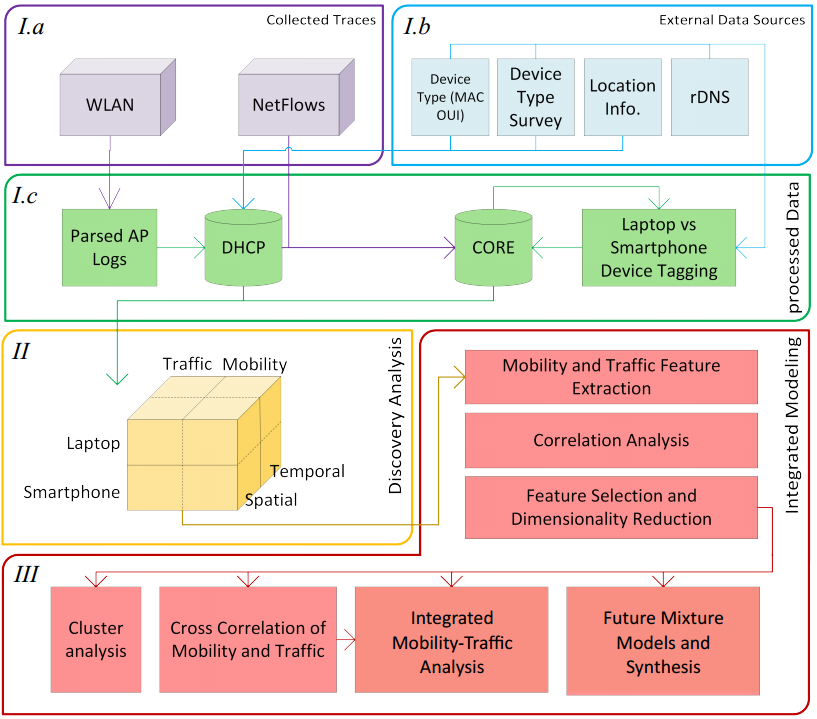
\includegraphics[width=0.65\textwidth]{img/FLAMeS.png}
% \caption{FLAMeS-System. \cite{Alipour2018}}
% \label{fig:flames}
% \end{figure}

\subsection{Datensammlung und Preprocessing}
\label{sec:phase1}

Die gesammelten Daten stammen aus zwei Quellen. Bei der ersten Quelle handelt es sich um WLAN-AP \footnote{Access-Point}-Logs,
welche an $1760$ APs in $138$ Gebäuden über $479$ Tage auf dem Campus einer Universität aufgezeichnet wurden. 
Die Daten stammen von insgesamt $316$\textsc{K} Geräten aus den Jahren $2011$ und $2012$. Jeder Eintrag enthält die 
MAC-Adresse des Geräts, dessen zugewiesene IP-Adresse, den AP, mit welchem das Gerät verbunden ist und einen Zeitstempel.
Die Orte der APs werden durch die Längen- und Breitengrade der Gebäude, in welchen sie sich befinden, mithilfe der Google Maps API
approximiert. Als weitere Quelle dienen Netflow \footnote{Ermöglicht Export von Informationen über den IP-Datenstrom eines 
Netzwerks. \cite{RFC3954}}-Logs, die im selben Netzwerk aus über $76$ Mrd. Einträgen in Netflow-Traces generiert werden.
Ein \textquote{Flow} entspricht einer konsekutiven Sequenz von Paketen
mit demselben Transportprotokoll, Start- und Ziel-IP und Port. \cite{Alipour2018}
Um die Daten aus den unterschiedlichen Quellen zu vereinen, matchen die Autoren die Netflow-Records 
durch das dynamische MAC-to-IP-Mapping mit den WLAN-Verbindungen aus den AP-Logs und ergänzen
die Ergebnisse mittels rDNS \footnote{Reverse DNS} durch Ort und Webseiten-Informationen.
Nachdem die Datenbasis geschaffen ist, geht es darum, die Geräte in Laptops und Smartphones zu klassifizieren.
Zunächst kann der Hersteller des Geräts mit der OUI \footnote{Organizationally Unique Identifier: 24-Bit-ID, 
die eindeutig den Hersteller identifiziert. \cite{RFC5342}} basierend auf den ersten drei Oktetten der MAC-Adresse identifiziert werden.
Da viele Hersteller lediglich einen Gerätetyp herstellen, können auf diese Weise bereits
$46 \%$ der Geräte klassifiziert werden. Die Heuristik, welche von den Autoren zur Klassifizierung verwendet wird,
prüft zusätzlich, ob ein Gerät \textit{admob.com} kontatktiert, eine sehr verbreitete Plattform für Werbung auf Mobilgeräten.
Ist dies der Fall, so wird dieses Gerät als Mobilgerät klassifiziert. Auf diese Weise können $86 \%$ der Geräte in den AP-Logs
und $97 \%$ der Netflow-Traces klassifiziert werden.
Die Autoren heben besonders hervor, dass diese Art der Geräteklassifizierung im Gegensatz zur Analyse von 
HTTP-Headern, welche möglicherweise zu noch genaueren Ergebnissen führt, die Privatsphäre der Nutzer wahrt.\newline
Wie man Abb. \ref{fig:traces} entnehmen kann, ist die Anzahl der Flows und das Gesamtvolumen des Datenverkehrs bei Laptops
erheblich größer als bei Smartphones, obwohl es insgesamt deutlich mehr verbundene Smartphones gibt. 
Die Spitzen treten erwartungsgemäß jeweils an Wochentagen auf. 
Die abrupte Abnahme der Netzwerkaktivität nach dem 25. ist im Beginn der vorlesungsfreien Zeit begründet.

\begin{figure}[H]
    \centering
    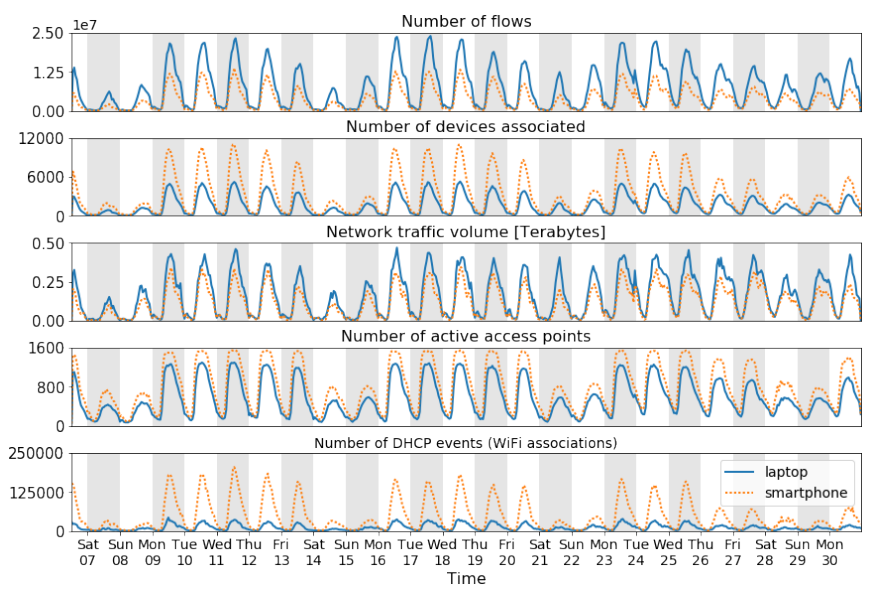
\includegraphics[width=0.55\textwidth]{img/traces.png}
    \caption{Kombinierte WLAN-AP- und Netflow-Traces. \cite{Alipour2018}}
    \label{fig:traces}
\end{figure}

\subsection{Mobilitätsanalyse}
\label{sec:phase2_a}

In diesem Abschnitt werden die Ergebnisse der Mobilitätsanalyse aus \cite{Alipour2018} zusammengefasst, in welcher es
um die zeitliche und räumliche Analyse der Mobilität der verschiedenen Gerätetypen geht.
Die Startzeiten von WLAN-Sessions stimmen in Gebäuden, in denen Vorlesungen stattfinden mit den Startzeiten der Vorlesungen überein.
In diesen Gebäuden fällt die Aktivität von Laptops nach dem Ende der Vorlesungszeiten stark, während die Aktivität von Mobilgeräten
noch etwas länger erhalten bleibt. Für die Bibliothek und soziale Einrichtungen auf dem Campus ist die Wahrscheinlichkeit
für neue Sessions später am Abend höher. Diese Ergebnisse treffen nur auf Wochentage zu, deren Ablauf durch
die Vorlesungszeiten eine gewisse Struktur erhält. Diese Struktur hat außerdem zur Folge, dass Stundenten, die an 
Vorlesungen teilnehmen, an Wochentagen einen eingeschränkteren Bewegungsradius haben. Die Autoren
analysieren die räumliche Ausbreitung der Geräte über einen Zeitraum von $6$ Monaten.
Nach einer initialen Phase von ca. einer Woche stabilisiert sich diese Ausbreitung. Für Laptops findet eine 
substanzielle Reduktion der Gesamtmobilität statt, während diese bei Smartphones nicht in einer solchen Deutlichkeit vorliegt.
Da Smartphones \textquote{always-on}-Geräte sind, ist es leichter, deren Mobilität zu erfassen, da sie auch an Orten
wie Bushaltestellen etc., an denen Laptops typischerweise nicht eingeschaltet sind, verbunden sind.
Dies ermöglicht eine genauere Erfassung der Mobilität dieser Geräte.
Außerdem wird die Anzahl der unterschiedlichen besuchten Gebäude eines Nutzers gezählt und ein bevorzugtes
Gebäude dieses Nutzers als jenes definiert, in welchem dieser an einem Tag die meiste Zeit verbringt.
Dazu werden die Session-Zeiten innerhalb eines Gebäudes aufsummiert.
Laptops besitzen etwas längere Aufenthaltszeiten und werden in der Regel verwendet, wenn Nutzer länger an einem Ort verweilen.

\subsection{Datenverkehranalyse}
\label{sec:phase2_b}

In diesem Abschnitt werden die Ergebnisse der zeitlichen und räumlichen Analyse des Datenverkehrs der verschiedenen Gerätetypen
aus \cite{Alipour2018} vorgestellt. Eine relevante Eigenschaft ist die Größe eines Flows, also die Summe der Bytes aller
Pakete eines Flows. An Wochentagen sind Smartphone-Flows durchschnittlich mehr als doppelt so groß wie Laptop-Flows
und auch an Wochenenden ändert sich dies nicht signifikant. Die durchschnittliche Paketgröße von Smartphone-Flows
ist ca. $50 \%$ größer als jene von Laptops. Im Median fällt die Größe der Pakete von Smartphones an Wochenenden, 
während diese bei Laptops gleich bleibt. Laptop-Flows zeigen zwischen Wochentagen und Wochenenden in Bezug auf die 
durchschnittliche Paketgröße keine signifikante Veränderung. Trotz kleinerer Flows generiert ein durchschnittlicher Laptop $2.7$
mal so viel Datenverkehr wie ein durchschnittliches Smartphone, weil ein Laptop für $3.7$ mal so viele Flows verantwortlich ist.
Ebenfalls aufschlussreich ist die Laufzeit eines Flows, wobei beide Gerätetypen erhöhte Mittelwerte an Wochenenden zeigen.
Da es zusätzlich weniger aktive Geräte an Wochenenden gibt, ist für die verbleibenden Geräte eine erhöhte Aktivität
zu beobachten. Smartphones zeigen insgesamt mehr extreme Phasen der Inaktivität, welche die Autoren unter anderem durch größere
Mobilität und Paketverluste erklären. Auch die verwendeten Protokolle sind von Interesse. 
TCP ist für $78.5 \%$ der Laptop-Flows verantwortlich und für $98.2 \%$ der Smartphone-Flows. 
Die höhere Präsenz von UDP bei Laptops ist zu erwarten, weil UDP-Verbindungen, die z.B. bei Multiplayer-Spielen, 
Video-Konferenzen und Filesharing auftreten, typischerweise weniger auf Mobilgeräten stattfinden. \cite{Alipour2018}
Außerdem wird die Last an den APs in sämtlichen Gebäuden täglich beobachtet. Dabei achten die Autoren darauf,
die Beobachtungen außerhalb der Klausurenphase zu tätigen, um Veränderungen im Verhalten der Nutzer zu vermeiden.
Es wird die tägliche Rate der Paket- und Flowankünfte an den APs betrachtet. Die Flowraten betragen im Median
$42$\textsc{K} bzw. $20$\textsc{K} für Laptops und Smartphones an Wochentagen und $7.5$\textsc{K} bzw. $0.5$\textsc{K}
an Wochenenden. Die durchschnittliche Anzahl von Laptop-Paketen, die täglich von APs verarbeitet werden,
ist $1.6$ mal größer als die von Smartphones. An Wochenenden wird ein großer Anteil der APs nicht verwendet,
was die Aussage einer geringeren Mobilität der Nutzer an Wochenenden unterstützt. \cite{Alipour2018}
Das tatsächliche Datenverkehr-Volumen der APs beträgt an durchschnittlichen Wochentagen für $90 \%$ der APs
weniger als $5$\textsc{GB} Laptop-Traffic ($2.5$\textsc{GB} an Wochenenden) und weniger als $3$\textsc{GB} Smartphone-Traffic
($1$\textsc{GB} an Wochenenden). Auch das Verhalten der Nutzer ist von Relevanz. An Wochentagen konsumieren $90 \%$ der 
Laptops weniger als $700$\textsc{MB}, während $90 \%$ der Smartphones weniger als $200$\textsc{MB} verbrauchen.
Ein ähnliches Bild ergibt sich bei der Paketrate. An Wochentagen generieren Laptops durchschnittlich $318$\textsc{K} Pakete, 
während Smartphones nur durchschnittlich $84$\textsc{K} Pakete am Tag generieren. 
An Wochenenden erhöht sich die Paketrate und der Datenkonsum der wenigen verbleibenden Laptops deutlich,
während bei den Smartphones nur leichte Veränderungen zu beobachten sind.
Weiterhin gut geeignet, um Unterschiede zwischen Laptops und Smartphones zu verdeutlichen, sind die tatsächlichen Aktivitätszeiten.
Dabei werden die Netflows herangezogen und nicht die WLAN-AP-Verbindungszeiten, denn dies ermöglicht es, \textquote{Idle}-Zeiten
von aktiven Zeiten zu unterscheiden. Laptops haben verglichen mit Smartphones $4$ mal höhere durchschnittliche Aktivitätszeiten.
Insgesamt sind über $90 \%$ der Laptops weniger als $3.5$ Stunden am Tag aktiv und $90 \%$ der Smartphones weniger als eine Stunde.\newline
Zusammenfassend kommen die Autoren zu dem Ergebnis, dass der Datenverkehr von Smartphones mehr \textquote{bursty} mit größeren Flows und kleinerer 
aktiver Dauer ist. Außerdem befinden sich an Wochenenden weniger Geräte auf dem Campus, aber jene, die verbleiben, sind überdurchschnittlich
aktiv und konsumieren überdurchschnittlich viele Daten. Insgesamt ist festzuhalten, dass Smartphones trotz größerer Flows etc. 
für insgesamt deutlich weniger Netzwerklast verantwortlich sind.

\subsection{Exkurs: Feature-Engineering}
\label{sec:digression}

Die Identifizierung relevanter Features ist essenziell, um Data-Mining-Algorithmen effektiv mit realen Daten zu verwenden.
Machine-Learning-Methoden haben Schwierigkeiten, mit großen Zahlen von Input-Features umzugehen, 
um diese Methoden dennoch effektiv anzuwenden, ist ein Preprocessing der Daten vonnöten. \cite{Kumar2014}
Dieser Preprocessing-Schritt geschieht in der integrierten Mobilitäts- und Datenverkehr-Analyse in \cite{Alipour2018},
welche in Abschnitt \ref{sec:phase3} besprochen wird, in Form von Feature-Selection. Feature-Selection ist der Prozess,
in welchem relevante Features von irrelevanten unterschieden werden. Die irrelevanten Features werden nicht betrachtet, 
was die Genauigkeit, Geschwindigkeit und Verständlichkeit der Methoden verbessert. \cite{Kumar2014} Irrelevante Features sind jene, 
die keine relevanten Informationen liefern und redundante Features liefern keine zusätzlichen Informationen.
Die betrachteten Features sollten dementsprechend weder irrelevant noch redundant sein.

\subsection{Integrierte Mobilitäts- und Datenverkehr-Modelle}
\label{sec:phase3}

In diesem Abschnitt geht es um den eigentlichen Kern von \cite{Alipour2018}, der Untersuchung, ob es einen Bedarf
für integrierte Mobilitäts- und Datenverkehr-Modelle gibt. Zur Identifikation der wichtigsten Features wird
mithilfe eines \textsc{CFS} \footnote{Correlation Feature Selection}-Algorithmus
Feature-Engineering (vgl. Abschnitt \ref{sec:digression}) betrieben. \textsc{CFS} ist eine Möglichkeit der Feature-Selection,
die auf Korrelationen basiert. Die zentrale Hypothese des Ansatzes ist, dass gute Teilmengen der Features jene Features enthalten,
die stark mit der Klasse, jedoch nicht untereinander korrelieren. \textsc{CFS} kombiniert diese Hypothese mit einem geeigneten
Maß der Korrelation und einer heuristischen Suche. \cite{Hall2000}
Bei den in \cite{Alipour2018} ermittelten Korrelationen handelt es sich um Pearson-Korrelationen.
Die \textquote{Pearson-Correlation}-Methode vergibt Werte zwischen $-1$ und $1$, wobei $0$ überhaupt keiner Korrelation
entspricht. Bei den Werten $1$ und $-1$ handelt es sich um totale positive bzw. negative Korrelationen.
Eine positive Korrelation zwischen zwei Features $A$ und $B$ liegt vor, wenn bei steigendem Wert für $A$
auch der Wert von $B$ steigt. Wohingegen bei einer negativen Korrelation bei einer Steigerung des Werts von $A$, 
der Wert von $B$ fällt. \cite{Nettleton2014}
\newline\newline\newline
\textbf{Korrelationen zwischen Mobilitäts- bzw. Datenverkehrmetriken}
\newline\newline
Der \textsc{CFS}-Algorithmus wird mit $8$ Mobilitäts-Features ausgeführt und selektiert $5$ Features, 
die für eine kombinierte Analyse geeignet sind. Für Laptops existiert z.B. an Wochentagen eine starke Korrelation ($0.96$)
zwischen der Zeit, welche im bevorzugten Gebäude verbracht wird und der Dauer der Session, jedoch nur eine schwache Korrelation
($0.1$) an Wochenenden, was darauf hindeutet, dass die meiste Onlinezeit am Wochenende im bevorzugten
Gebäude verbracht wird. \cite{Alipour2018} Die vollständigen Ergebnisse zu Korrelationen der Mobilitätsmetriken können in
Abb. \ref{fig:mobility_correlations} nachvollzogen werden.\newline
Bezüglich der Eigenschaften des Datenverkehrs wird der \textsc{CFS}-Algorithmus mit $19$ Features ausgeführt, von denen $11$
selektiert werden. Auch beim Datenverkehr existieren einige Korrelationen, die in Abb. \ref{fig:traffic_correlations} nachvollzogen werden können.
Die wohl interessanteste Erkenntnis ist allerdings, dass die Aktivitätszeiten und die Anzahl von Flows und Paketen nur
schwach korrelieren, was bedeutet, dass Nutzer, die länger online sind, nicht notwendigerweise mehr Datenverkehr erzeugen. \cite{Alipour2018}
\newline\newline
Ein wichtiger Schritt in Richtung integrierter Modelle ist die Analyse der Korrelationen
zwischen beiden Dimensionen (Mobilität und Datenverkehr) basierend auf der Teilmenge der Features bzw. Metriken,
die vom \textsc{CFS}-Algorithmus selektiert werden. Die entsprechenden Ergebnisse aus \cite{Alipour2018} lassen sich wie 
folgt zusammenfassen. Smartphones haben erwartungsgemäß hohe Scores bei den Mobilitätsmetriken (Bewegungsradius,
Anzahl besuchter unterschiedlicher Gebäude etc.), besitzen eine
insgesamt kleinere Anzahl von Flows und sorgen für weniger Datenverkehr, aber produzieren im Durchschnitt größere Flows.
Für Laptops gilt an Wochenenden, je mehr Zeit in bevorzugten Gebäuden verbracht wird, desto größer die Gesamtaktivitätszeit
und Flow-Anzahl. Dieser Effekt existiert in abgeschwächter Form auch bei Smartphones. 
An Wochentagen existieren diese Korrelationen nicht. Die exakten Ergebnisse sind in Abb. \ref{fig:mobility_traffic_correlations}
dargestellt. Mittels Machine-Learning untersuchen die Autoren, wie sich Mobilitäts- und Datenverkehr-Features zwischen
Smartphones und Laptops unterscheiden. Anschließend wird nach natürlichen konvexen Clustern von Nutzern bzw. Geräten im
Datensatz gesucht. Diese Schritte verifizieren, dass die Unterschiede der Mobilitäts- und Datenverkehr-Charakteristiken
zwischen den Gerätetypen signifikant sind.\newline
% \textbf{Supervised Classification}\newline
Die Autoren verwenden Support-Vector-Maschinen (SVM) auf verschiedenen Teilmengen von Features, 
um die Zulässigkeit der Gerätetyp-Inferenz und die Beziehung zwischen Mobilitäts- und Datenverkehr-Charakteristiken
zu untersuchen. Insgesamt wird die Genauigkeit verschiedener Modelle analysiert. Dabei stellt sich heraus,
dass kombinierte Modelle, welche sowohl den Datenverkehr als auch die Mobilität berücksichtigen, 
mit $\approx 81 \%$ genauer sind als isolierte Modelle (Mobilität $\approx 65 \%$, Datenverkehr $\approx 79 \%$).
Außerdem erhöht sich die Genauigkeit auf $\approx 86 \%$, wenn zudem zwischen Wochentagen und Wochenenden differenziert wird.
% \newline\newline
% \textbf{Unsupervised Clustering}\newline
Um natürliche konvexe Cluster zu untersuchen, verwenden sie einen $k$-Means-Algorithmus.
Werden ausschließlich Mobilitäts-Features genutzt, so werden ca. $60 \%$ der Geräte korrekt geclustert.
Ein ausschließlicher Fokus auf Datenverkehr-Features führt zu einer Genauigkeit von $81.2 \%$.
Bei einer Kombination der Features erhöht sich die Genauigkeit leicht auf $81.5 \%$.
\newline\newline\newline
\textbf{Kombiniertes Modell}
\newline\newline
Um erste Traces basierend auf den Datensätzen zu generieren, trainieren die Autoren schließlich Gaussian-Mixture-Models (GMM) mit
kombinierten Features. Anschließend verwenden sie Kolmogorov-Smirnov (KS) Statistik, um die generierten
Samples mit Echtdaten zu vergleichen. Das kombinierte Modell produziert Samples, dessen Datenverkehr-Features
den Originaldaten besser entsprechen als ein GMM, welches ausschließlich mit Datenverkehr-Features trainiert wurde,
was darauf hindeutet, dass eine Beziehung zwischen Mobilität und Datenverkehr besteht. \cite{Alipour2018}
Allerdings bringt das GMM des kombinierten Modells in Bezug auf Mobilitäts-Features verglichen mit
dem Modell, welches ausschließlich mit Mobilitäts-Features trainiert wurde, keine Verbesserung.

\subsection{Zusammenfassung}
\label{sec:summary}

In \cite{Alipour2018} geht es im Kern um die Frage, ob es sinnvoll ist, Modelle zu entwickeln, die sowohl
Mobilitäts- als auch Datenverkehrcharakteristiken eines Drahtlosnetzwerks berücksichtigen.
Die Autoren stellen ein Framework vor, um die Datensätze eines bestehenden Netzwerks dahingehend zu analysieren.
Zunächst geht es dabei um Geräteklassifizierung und anschließend um eine Untersuchung der Mobilitäts-
und Datenverkehr-Metriken, wobei die verschiedenen Gerätetypen über Raum und Zeit hinweg miteinander verglichen werden.
Nach dem Hervorheben signifikanter Unterschiede zwischen den Gerätetypen, wird mittels Machine-Learning ein kombiniertes Modell
trainiert. Dieses Modell bildet die Unterschiede in den Metriken besser ab als isolierte Modelle.
Insgesamt sehen die Autoren ein signifikantes Potenzial integrierter Modelle, welche die Unterschiede und Beziehungen 
von Features zwischen Gerätetypen, Zeit und Ort besser repräsentieren als gengenwärtige Modelle. 
Somit werden die eingangs erwähnten Fragestellungen in einer Weise beantwortet, die zukünftige Forschung zu
integrierten Modellen nahelegt. Da viele der Erkenntnisse von aktuellen Modellen nicht berücksichtigt werden, 
liefert die Veröffentlichung wichtige Grundlagen für das Design zukünftiger Modelle.

\vfill
\pagebreak

\section{Fazit und Ausblick}
\label{sec:conclusion}

Da ein Modell eine Repräsentation bestimmter Aspekte eines real existierenden Konzepts ist,
ist es von zentraler Bedeutung, diese Aspekte mit Bedacht zu wählen, sodass möglichst nur
Aspekte modelliert werden, welche tatsächlich relevant sind. Gleichzeitig sollten sämtliche relevanten
Aspekte Teil des Modells sein. Übertragen auf Netzwerkmodelle sind die bisher existierenden Modelle
basierend auf den Erkenntnissen aus \cite{Alipour2018} nicht detailliert genug. Es werden entweder
Datenverkehr- oder Mobilitätscharakteristiken modelliert, jedoch nicht das Zusammenspiel beider Faktoren.
Die betrachtete Veröffentlichung liefert demnach einen wichtigen Anstoß zur Entwicklung besserer Netzwerkmodelle.
Die Autoren von \cite{Alipour2018} haben eine erweiterte Version des Papers veröffentlicht,
in welcher sie tiefer auf bestimmte zuvor betrachtete Aspekte eingehen und weitere Erkenntnisse in Bezug
auf das Design und die Parametrisierung von zukünftigen Modellen eingehen.
Die Details können im Rahmen dieser Ausarbeitung nicht mehr erörtert werden, es ist jedoch wichtig, zu erwähnen,
dass die Autoren auf zusätzliche Faktoren hinweisen, so können Mobilität und Datenverkehr nicht nur
zwischen den Gerätetypen unterschieden werden, sondern zusätzlich zwischen unterschiedlichen Nutzergruppen.
Die Tatsache, dass unter anderem Alter und Geschlecht eines Nutzers einen Einfluss auf dessen erzeugten Datenverkehr haben können,
wird auch in \cite{Oliveira2014} thematisiert. Dort wird darauf hingewiesen, dass es wichtig ist,
zu berücksichtigen, in welchem kulturellen Kontext Daten aufgezeichnet werden.\newline
Auch wenn die Autoren von \cite{Alipour2018} die Konzeption und Validierung eines konkreten Modells
zukünftiger Forschung überlassen, liefern sie wichtige Erkenntnisse für den Entwurf von integrierten Modellen,
die für zahlreiche praktische Anwendungen von Relevanz sein können.
Bereits das alltägliche Beispiel der Person, die ihren Gang verlangsamt um eine empfangene Nachricht zu lesen,
verdeutlicht, dass Mobilität und Datenverkehr bei Mobilgeräten nicht isoliert betrachtet werden sollten.
In \cite{Alipour2018} wird diese intuitive Idee eines Zusammenhangs bestätigt.\newline
Die Relevanz von Simulationen der Mobilität von Geräten bzw. Benutzern innerhalb eines Netzwerks
ist bereits ausführlich diskutiert worden. Um möglichst akurate Simulationen durchzuführen, wäre es erstrebenswert,
die Mobilität von realen Benutzern möglichst genau vorherzusagen. Mit dieser Vorhersagbarkeit haben sich die Autoren
von \cite{Alipour2018} in einer weiteren Veröffentlichung mit dem Titel \textquote{Practical Prediction of Human
Movements Across Device Types and Spatiotemporal Granularities}\cite{Alipour2019} aus diesem Jahr beschäftigt.
Sie gelangen darin zu dem Schluss, dass die Bewegung von Laptops oder allgemein \textquote{sit-to-use}-Geräten
erheblich besser vorherzusagen ist als jene von Smartphones bzw. Mobilgeräten.
Aufgrund signifikanter Korrelationen zwischen Vorhersagegenauigkeit, Mobilitäts- und Datenverkehr-Features
planen die Autoren den Nutzen der Vorhersagegenauigkeit als Feature in integrierten Mobilitäts- und Datenverkehr-Modellen
weiter zu untersuchen.\newline
Bei der möglichst realistischen Modellierung der Netzwerkaktivität handelt es sich um ein aktives Forschungsfeld,
weshalb in Zukunft weitere Betrachtungen und konkretere Ansätze kombinierter Modelle zu erwarten sind.

\vfill
\pagebreak

%Bibliographie
\addcontentsline{toc}{section}{Literatur}
\bibliographystyle{IEEEtranSA}
%\bibliographystyle{acm}
\bibliography{sources.bib}

\vfill
\pagebreak

\begin{appendix}
\section{Anhang}

\begin{figure}[H]
    \centering
    \begin{subfigure}[b]{0.45\textwidth}
        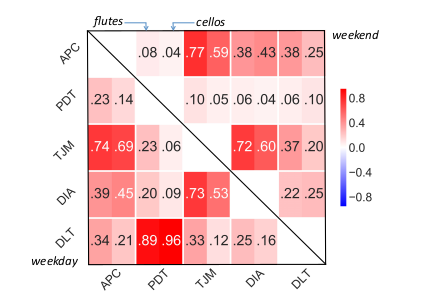
\includegraphics[width=0.7\textwidth]{img/mobility_correlations.png}
        \caption{Korrelationen \cite{Alipour2018}}
    \end{subfigure}
    \hfill
    \begin{subfigure}[b]{0.45\textwidth}
        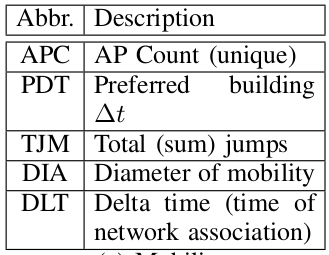
\includegraphics[width=0.55\textwidth]{img/mobility_metrics.png}
        \caption{Metriken \cite{Alipour2018}}
    \end{subfigure}
    \caption{Korrelationen zwischen Mobilitätsmetriken.}
    \label{fig:mobility_correlations}
\end{figure}

\begin{figure}[H]
    \centering
    \begin{subfigure}[b]{0.45\textwidth}
        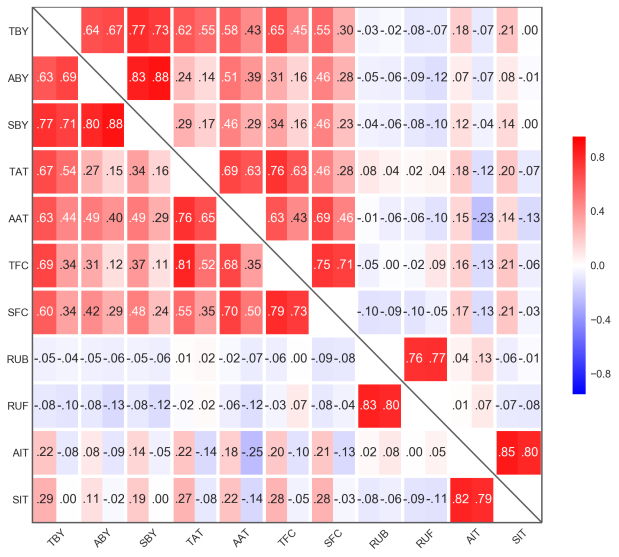
\includegraphics[width=0.8\textwidth]{img/traffic_correlations.png}
        \caption{Korrelationen \cite{Alipour2018}}
    \end{subfigure}
    \hfill
    \begin{subfigure}[b]{0.45\textwidth}
        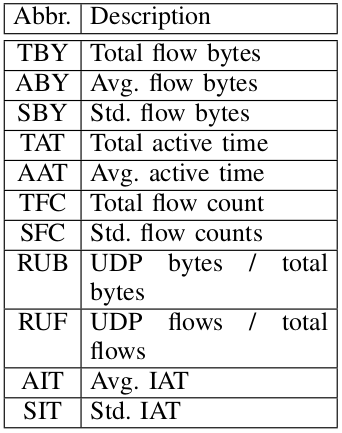
\includegraphics[width=0.55\textwidth]{img/traffic_metrics.png}
        \caption{Metriken \cite{Alipour2018}}
    \end{subfigure}
    \caption{Korrelationen zwischen Datenverkehrmetriken.}
    \label{fig:traffic_correlations}
\end{figure}

\begin{figure}[H]
    \centering
    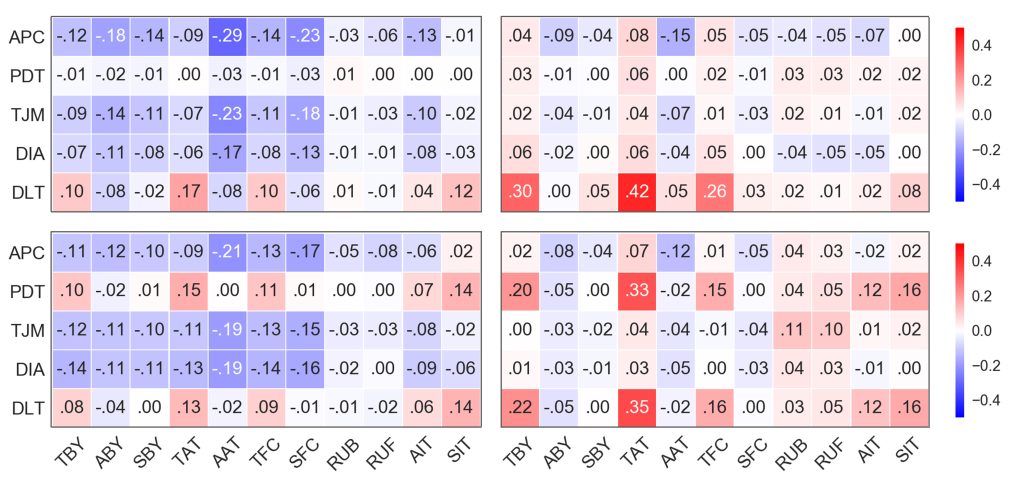
\includegraphics[width=0.55\textwidth]{img/mobility_traffic_correlations.png}
    \caption{Korrelationen zwischen Mobilitäts- und Traffic-Features (Wochentage oben, Wochendenden unten,
    Smartphones links, Laptops rechts). \cite{Alipour2018}}
    \label{fig:mobility_traffic_correlations}
\end{figure}

\end{appendix}

\end{document}
